\documentclass[12pt]{article}
\usepackage{amsmath}
\usepackage{graphicx}
\usepackage{hyperref}
\usepackage{listings}
\usepackage{color}
\usepackage{pythonhighlight}
\usepackage{caption}
\usepackage{float}
\captionsetup{labelformat=empty}

\title{Operating System Course Report - First Half of the Semester}
\author{A class}
\date{\today}

\begin{document}

\maketitle
\newpage

\tableofcontents
\newpage

\section{Introduction}
This report summarizes the topics covered during the first half of the Operating System course. It includes theoretical concepts, practical implementations, and assignments. The course focuses on the fundamentals of operating systems, including system architecture, process management, CPU scheduling, and deadlock handling.

\section{Course Overview}
\subsection{Objectives}
The main objectives of this course are:
\begin{itemize}
    \item To understand the basic components and architecture of a computer system.
    \item To learn process management, scheduling, and inter-process communication.
    \item To explore file systems, input/output management, and virtualization.
    \item To study the prevention and handling of deadlocks in operating systems.
\end{itemize}

\subsection{Course Structure}
The course is divided into two halves. This report focuses on the first half, which covers:
\begin{itemize}
    \item Basic Concepts and Components of Computer Systems
    \item System Performance and Metrics
    \item System Architecture of Computer Systems
    \item Process Description and Control
    \item Scheduling Algorithms
    \item Process Creation and Termination
    \item Introduction to Threads
    \item File Systems
    \item Input and Output Management
    \item Deadlock Introduction and Prevention
    \item User Interface Management
    \item Virtualization in Operating Systems
\end{itemize}

\section{Topics Covered}

\subsection{Basic Concepts and Components of Computer Systems}
This section explains the fundamental components that make up a computer system, including the CPU, memory, storage, and input/output devices.

\subsection{System Performance and Metrics}
This section introduces various system performance metrics used to measure the efficiency of a computer system, including throughput, response time, and utilization.

\subsection{System Architecture of Computer Systems}
Describes the architecture of modern computer systems, focusing on the interaction between hardware and the operating system.

\subsection{Process Description and Control}
Processes are a central concept in operating systems. This section covers:
    \subsubsection{\textit{Process Description}}
    Menurut Silberschatz, Galvin, dan Gagne (2009), proses adalah sebuah
    program yang sedang dijalankan pada komputer. Setiap proses membutuhkan
    sumber daya, seperti CPU, memori, dan perangkat \textit{input/output},
    untuk bisa berfungsi dengan baik. Komputer harus mengelola berbagai
    proses agar semua program dapat berfungsi dengan baik. Dalam pengelolaan ini,
    setiap proses memiliki \textit{process state} dan \textit{Process Control Block}
    (PCB) yang membantu sistem untuk mengawasi dan mengatur kondisi serta informasi 
    penting mengenai proses tersebut.
    
    \subsubsection{Process States and State Transitions}
        \begin{figure}[h]
            \centering
            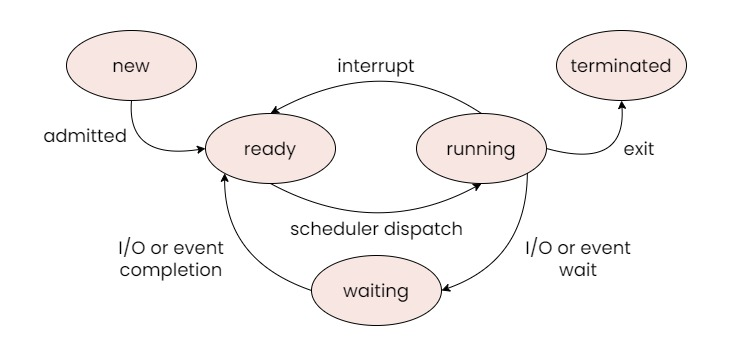
\includegraphics[width=0.8\textwidth]{asset/process-state.jpg}
            \caption{Gambar 1: \textit{Process states and state transitions}}
            \label{fig:process_state}
        \end{figure}

        Dalam sistem operasi (OS), manajemen cara program berjalan dan
        berinteraksi dengan sumber daya sistem sangat penting untuk
        kinerja yang efisien. \textit{The 5-process-state model} adalah
        kerangka dasar yang digunakan oleh OS untuk mengategorikan
        dan mengendalikan perilaku proses.

        Model ini membagi siklus hidup sebuah proses menjadi lima status
        yang berbeda, masing-masing mewakili tahap yang berbeda dalam eksekusinya.
        Memahami status-status ini membantu dalam mengoptimalkan penggunaan sumber
        daya, memastikan \textit{multitasking} yang lancar, dan menjaga stabilitas
        sistem. (GeeksForGeeks, 2024)

        Siklus hidup proses dalam sistem operasi terdiri dari beberapa status,
        seperti yang terlihat pada gambar di atas. Status-status tersebut meliputi:
        \begin{itemize}
            \item \textbf{\textit{New}}:
                Status ini menunjukkan bahwa proses baru saja dibuat dan sedang menunggu
                untuk dimasukkan dalam daftar proses yang siap dijalankan. Proses akan
                berada dalam status ini hingga sistem menerima proses tersebut.
            \item \textbf{\textit{Ready}}:
                Setelah proses diterima, proses akan berpindah ke status \textit{ready}.
                Di sini, proses sudah siap untuk dieksekusi namun harus menunggu hingga
                \textit{scheduler} memilihnya.
            \item \textbf{\textit{Running}}:
                Setelah mendapatkan jadwal, proses akan berpindah dari status \textit{ready}
                ke \textit{running}. Pada status ini, proses sedang dieksekusi oleh CPU,
                yang berarti ia sedang aktif melakukan tugasnya.
            \item \textbf{\textit{Waiting}}:
                Proses dapat berpindah ke status \textit{waiting} ketika sedang menunggu
                operasi I/O atau suatu \textit{event} tertentu. Status ini menunjukkan
                bahwa proses membutuhkan \textit{input} dari perangkat keras atau menunggu
                \textit{event} tertentu sebelum dapat melanjutkan eksekusi.    
            \item \textbf{\textit{Terminated}}:
                Setelah eksekusi selesai, proses akan berpindah ke status \textit{terminated},
                Pada tahap ini, proses tidak lagi menjadi bagian dari sistem.
        \end{itemize}
        Transisi antar status tersebut meliputi:
        \begin{itemize}
            \item \textbf{\textit{Admitted}}:
                Ketika sebuah proses baru dibuat, ia akan berpindah dari status \textit{new} ke
                \textit{ready} setelah diterima oleh sistem operasi. Ini menandakan bahwa proses
                tersebut sudah siap untuk berpindah ke status berikutnya.
            \item \textbf{\textit{Scheduler Dispatch}}:
                Ketika CPU siap untuk mengeksekusi proses, \textit{scheduler} akan memindahkan
                proses dari status \textit{ready} ke \textit{running}.  Ini menandakan bahwa
                proses tersebut sedang dieksekusi.
            \item \textbf{I/O or \textit{Event Wait}}:
                Ketika proses membutuhkan operasi I/O atau menunggu suatu \textit{event},
                proses akan berpindah dari \textit{running} ke \textit{waiting}.
            \item \textbf{I/O or \textit{Event Completion}}:
                Setelah operasi I/O atau kejadian selesai, proses yang berada di status
                \textit{waiting} akan berpindah kembali ke status \textit{ready}.
            \item \textbf{\textit{Interrupt}}:
                Jika proses yang sedang berjalan terganggu (misalnya terganggu oleh
                \textit{scheduler} untuk memberikan giliran kepada proses lain), 
                proses akan berpindah dari \textit{running} ke \textit{ready}.
            \item \textbf{\textit{Exit}}:
                Ketika proses selesai dieksekusi, ia akan berpindah dari \textit{running}
                ke \textit{terminated}.
        \end{itemize}

        \subsubsection {\textit{Process Control Block} (PCB)}

        \subsubsection {\textit{Process Control}}

    \begin{thebibliography}{9}
    \bibitem{Silberschatz2009} 
    Silberschatz, A., Galvin, P. B., \& Gagne, G. (2009). \textit{Operating System Concepts} (8th ed.).Hoboken, NJ: Wiley.
    \bibitem{GeeksForGeeks2024} 
    GeeksForGeeks. (2024, 22 Juli). \textit{5 State Process Model in Operating System}. Diakses pada 10 Oktober 2024, dari \url{https://www.geeksforgeeks.org/5-state-process-model-in-operating-system/}.    
    \end{thebibliography}

\subsection{Scheduling Algorithms}
This section covers:
\begin{itemize}
    \item First-Come, First-Served (FCFS)
    \item Shortest Job Next (SJN)
    \item Round Robin (RR)
\end{itemize}
It explains how these algorithms are used to allocate CPU time to processes.

\subsection{Process Creation and Termination}
Details how processes are created and terminated by the operating system, including:
\begin{itemize}
    \item Process spawning
    \item Process termination conditions
\end{itemize}

\subsection{Introduction to Threads}
This section introduces the concept of threads and their relation to processes, covering:
\begin{itemize}
    \item Single-threaded vs. multi-threaded processes
    \item Benefits of multithreading
\end{itemize}

\begin{figure}[h]
    \centering
    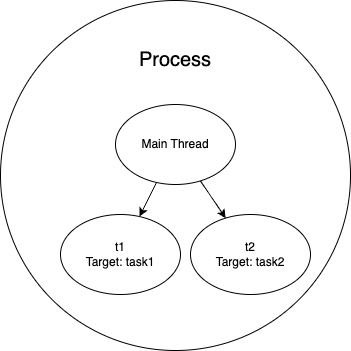
\includegraphics[width=0.5\textwidth]{asset/example.png}  % Sesuaikan nama file dan ukurannya
    \caption{Ini adalah gambar contoh dari multithreading.}
    \label{fig:contoh_gambar}
\end{figure}

Seperti yang terlihat pada Gambar \ref{fig:contoh_gambar}, inilah cara menambahkan gambar dengan keterangan.

\subsection{File Systems}
File systems provide a way for the operating system to store, retrieve, and manage data. This section explains:
\begin{itemize}
    \item File system structure
    \item File access methods
    \item Directory management
\end{itemize}

\subsection{Input and Output Management}
Input and output management is key for handling the interaction between the system and external devices. This section includes:
\begin{itemize}
    \item Device drivers
    \item I/O scheduling
\end{itemize}

\subsection{Deadlock Introduction and Prevention}
Explores the concept of deadlocks and methods for preventing them:
\begin{itemize}
    \item Deadlock conditions
    \item Deadlock prevention techniques
\end{itemize}

\subsection{User Interface Management}
This section discusses the role of the operating system in managing the user interface. Topics covered include:
\begin{itemize}
    \item Graphical User Interface (GUI)
    \item Command-Line Interface (CLI)
    \item Interaction between the user and the operating system
\end{itemize}

\subsection{Virtualization in Operating Systems}
Virtualization allows multiple operating systems to run concurrently on a single physical machine. This section explores:
\begin{itemize}
    \item Concept of virtualization
    \item Hypervisors and their types
    \item Benefits of virtualization in modern computing
\end{itemize}

\section{Assignments and Practical Work}
\subsection{Assignment 1: Process Scheduling}
Students were tasked with implementing various process scheduling algorithms (e.g., FCFS, SJN, and RR) and comparing their performance under different conditions.
    \subsubsection{Group 1}
\begin{python}
class Process:
    def __init__(self, pid, arrival_time, burst_time):
        self.pid = pid
        self.arrival_time = arrival_time
        self.burst_time = burst_time
        self.completion_time = 0
        self.turnaround_time = 0
        self.waiting_time = 0
\end{python}

        \begin{table}[htbp] % Optional: For floating position
            \centering
            \begin{tabular}{|c|c|c|} % Defines number of columns and alignment (c = center, l = left, r = right). '|' creates vertical lines.
            \hline
            Header 1 & Header 2 & Header 3 \\ % Column headers
            \hline
            Row 1, Column 1 & Row 1, Column 2 & Row 1, Column 3 \\ % First row of data
            \hline
            Row 2, Column 1 & Row 2, Column 2 & Row 2, Column 3 \\ % Second row of data
            \hline
            \end{tabular}
            \caption{Your table caption} % Optional: For adding a caption
            \label{tab:your_label} % Optional: For cross-referencing the table
        \end{table}

        \subsubsection{Group 4}
        \textbf{Pertanyaan: }

        Implementasikan algoritma \textit{First-Come, First-Served} (FCFS), \textit{Shortest Job Next} (SJN), dan \textit{Round Robin} (RR) dengan \textit{time quantum} = 4 untuk menghitung waktu tunggu (\textit{waiting time}) setiap proses serta rata-rata waktu tunggu proses berikut:
        \begin{table}[htbp] % Optional: For floating position
            \centering
            \begin{tabular}{|c|c|} % Defines number of columns and alignment (c = center, l = left, r = right). '|' creates vertical lines.
            \hline
            \textbf{Process ID} & \textbf{Burst Time (ms)} \\ 
            \hline
            P1 & 5 \\ 
            \hline
            P2 & 3 \\
            \hline
            P3 & 8 \\
            \hline
            P4 & 6 \\ 
            \hline
            \end{tabular}
                        \caption{Tabel 1: \textit{Process ID and their respective Burst Time}}
            \label{tab:process_burst_time} 
        \end{table}

        \noindent Dari ketiga algoritma tersebut, algoritma mana yang memiliki waktu tunggu rata-rata (\textit{average waiting time}) yang paling rendah?\\

        \noindent \textbf{Jawaban: }

        \noindent Untuk menjawab soal tersebut kita dapat menggunakan kode di bawah ini
\begin{python}
# Fungsi untuk algoritma First-Come, First-Served (FCFS)
def fcfs(processes):
    print("\nFirst-Come, First-Served (FCFS)")
    waiting_time = 0
    total_waiting_time = 0
    for p in processes:
        print(f"Process {p[0]} | Burst Time: {p[1]} | Waiting Time: {waiting_time}")
        total_waiting_time += waiting_time
        waiting_time += p[1]
    avg_waiting_time = total_waiting_time / len(processes)
    print(f"Average Waiting Time: {avg_waiting_time:.2f}")
    return avg_waiting_time

# Fungsi untuk algoritma Shortest Job Next (SJN)
def sjn(processes):
    print("\nShortest Job Next (SJN)")
    processes_sjn = sorted(processes, key=lambda x: x[1])  # Urutkan berdasarkan Burst Time
    waiting_time = 0
    total_waiting_time = 0
    for p in processes_sjn:
        print(f"Process {p[0]} | Burst Time: {p[1]} | Waiting Time: {waiting_time}")
        total_waiting_time += waiting_time
        waiting_time += p[1]
    avg_waiting_time = total_waiting_time / len(processes_sjn)
    print(f"Average Waiting Time: {avg_waiting_time:.2f}")
    return avg_waiting_time

# Fungsi untuk algoritma Round Robin (RR)
def round_robin(processes, quantum):
    print("\nRound Robin (RR)")
    remaining_burst_time = [p[1] for p in processes]
    waiting_time = [0] * len(processes)
    t = 0  # Waktu saat ini

    while True:
        done = True
        for i in range(len(processes)):
            if remaining_burst_time[i] > 0:
                done = False
                if remaining_burst_time[i] > quantum:
                    t += quantum
                    remaining_burst_time[i] -= quantum
                else:
                    t += remaining_burst_time[i]
                    waiting_time[i] = t - processes[i][1]
                    remaining_burst_time[i] = 0
        if done:
            break

    for i, p in enumerate(processes):
        print(f"Process {p[0]} | Burst Time: {p[1]} | Waiting Time: {waiting_time[i]}")
    avg_waiting_time = sum(waiting_time) / len(processes)
    print(f"Average Waiting Time: {avg_waiting_time:.2f}")
    return avg_waiting_time

# Daftar proses dengan format: [Process ID, Burst Time]
processes = [[1, 5], [2, 3], [3, 8], [4, 6]]

# Panggil fungsi untuk setiap algoritma scheduler
avg_fcfs = fcfs(processes)
avg_sjn = sjn(processes)
avg_rr = round_robin(processes, quantum=4)

# Mencari algoritma dengan rata-rata waktu tunggu terendah
min_avg_time = min(avg_fcfs, avg_sjn, avg_rr)
if min_avg_time == avg_fcfs:
    best_algorithm = "First Come, First Serve"
elif min_avg_time == avg_sjn:
    best_algorithm = "Shortest Job Next"
else:
    best_algorithm = "Round Robin"

print(f"\nAlgoritma dengan rata-rata waktu tunggu paling rendah adalah {best_algorithm} dengan rata-rata waktu tunggu sebesar {min_avg_time:.2f}.")
\end{python}
        \noindent \textbf{Output Kode:}
        \begin{figure}[h]
            \centering
            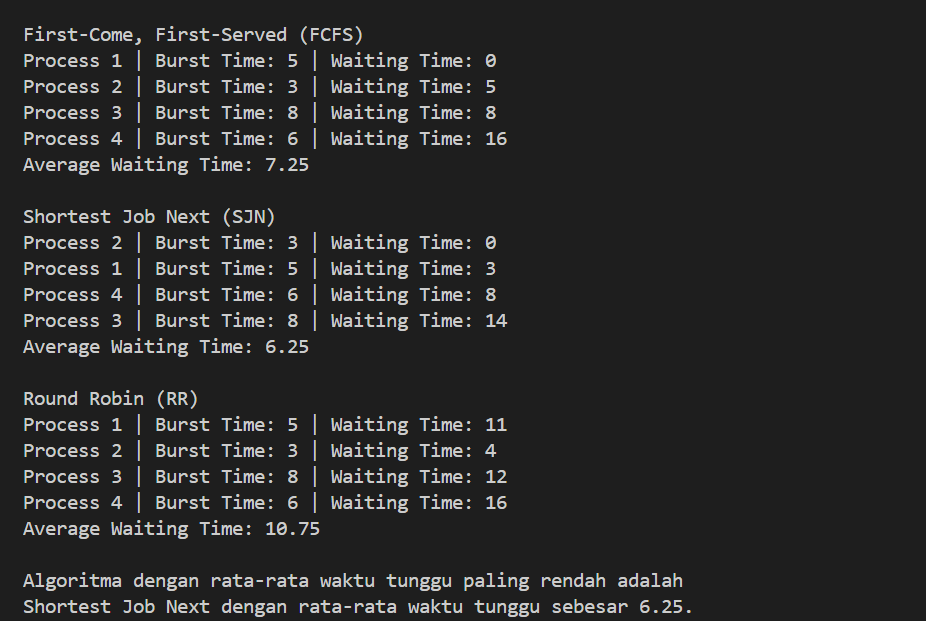
\includegraphics[width=0.9\textwidth]{asset/a1-output.png}
            \caption{Gambar 2: \textit{Output of Scheduling Algorithm Program}}
            \label{fig:a1-output}
        \end{figure}

\subsection{Assignment 2: Deadlock Handling}
In this assignment, students were asked to simulate different deadlock scenarios and explore various prevention methods.

\subsection{Assignment 3: Multithreading and Amdahl's Law}
This assignment involved designing a multithreading scenario to solve a computationally intensive problem. Students then applied **Amdahl's Law** to calculate the theoretical speedup of the program as the number of threads increased.

\subsection{Assignment 4: Simple Command-Line Interface (CLI) for User Interface Management}
Students were tasked with creating a simple **CLI** for user interface management. The CLI should support basic commands such as file manipulation (creating, listing, and deleting files), process management, and system status reporting.
\subsubsection{Group 4}
\noindent \textbf{Pertanyaan: }
Buatlah sebuah program Python yang berfungsi sebagai CLI sederhana untuk manajemen antarmuka pengguna! Program tersebut harus mendukung perintah dasar seperti manipulasi \textit{file} (membuat, menampilkan daftar, dan menghapus \textit{file}) serta pelaporan status sistem. \\

\noindent \textbf{Jawaban: }
\begin{python}
import os
import platform

# Membuat file baru dengan nama yang diberikan
def create_file(filename):
    with open(filename, 'w') as f:
        pass
    print(f"File '{filename}' created successfully.")

# Menampilkan daftar file dari sebuah direktori
def list_files(directory='.'):
    try:
        files = os.listdir(directory)
        if files:
            print("Files in directory:", directory)
            for file in files:
                print(f"- {file}")
        else:
            print(f"No files found in directory: {directory}")
    except FileNotFoundError:
        print(f"Directory '{directory}' not found.")

# Menghapus file dengan nama yang diberikan
def delete_file(filename):
    if os.path.isfile(filename):
        os.remove(filename)
        print(f"File '{filename}' deleted successfully.")
    else:
        print(f"File '{filename}' not found.")

# Menampilkan status sistem sederhana
def show_system_status():
    print(f"Operating System: {platform.system()} {platform.release()}")
    print(f"CPU Count: {os.cpu_count()}")

# Fungsi utama
def main():
    while True:
        print("\nCLI Simple Management Tool")
        print("1. Create File")
        print("2. List Files")
        print("3. Delete File")
        print("4. Show System Status")
        print("5. Exit")
        choice = input("Enter your choice (1-5): ")

        if choice == '1':
            filename = input("Enter the name of the file to create: ")
            create_file(filename)
        elif choice == '2':
            directory = input("Enter the directory to list files (default is current directory): ") or '.'
            list_files(directory)
        elif choice == '3':
            filename = input("Enter the name of the file to delete: ")
            delete_file(filename)
        elif choice == '4':
            show_system_status()
        elif choice == '5':
            print("You have successfully exited the CLI.")
            break
        else:
            print("Invalid choice, please select a number between 1 and 5.")

# Eksekusi program utama
if __name__ == "__main__":
    main()
\end{python}

        \noindent Berikut adalah \textit{output} dari program CLI yang dijalankan di \textit{command line}.
        \begin{figure}[htbp]
            \centering
            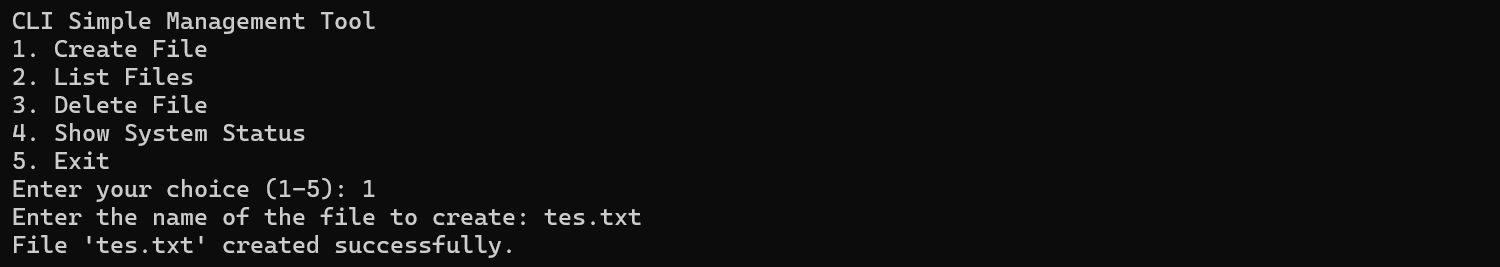
\includegraphics[width=0.9\textwidth]{asset/a4-output-1.png}
            \caption{Gambar 3: Membuat \textit{file} dengan nama 'tes.txt'}
            \label{fig:a4-output-1}
        \end{figure}
        \begin{figure}[htbp]
            \centering
            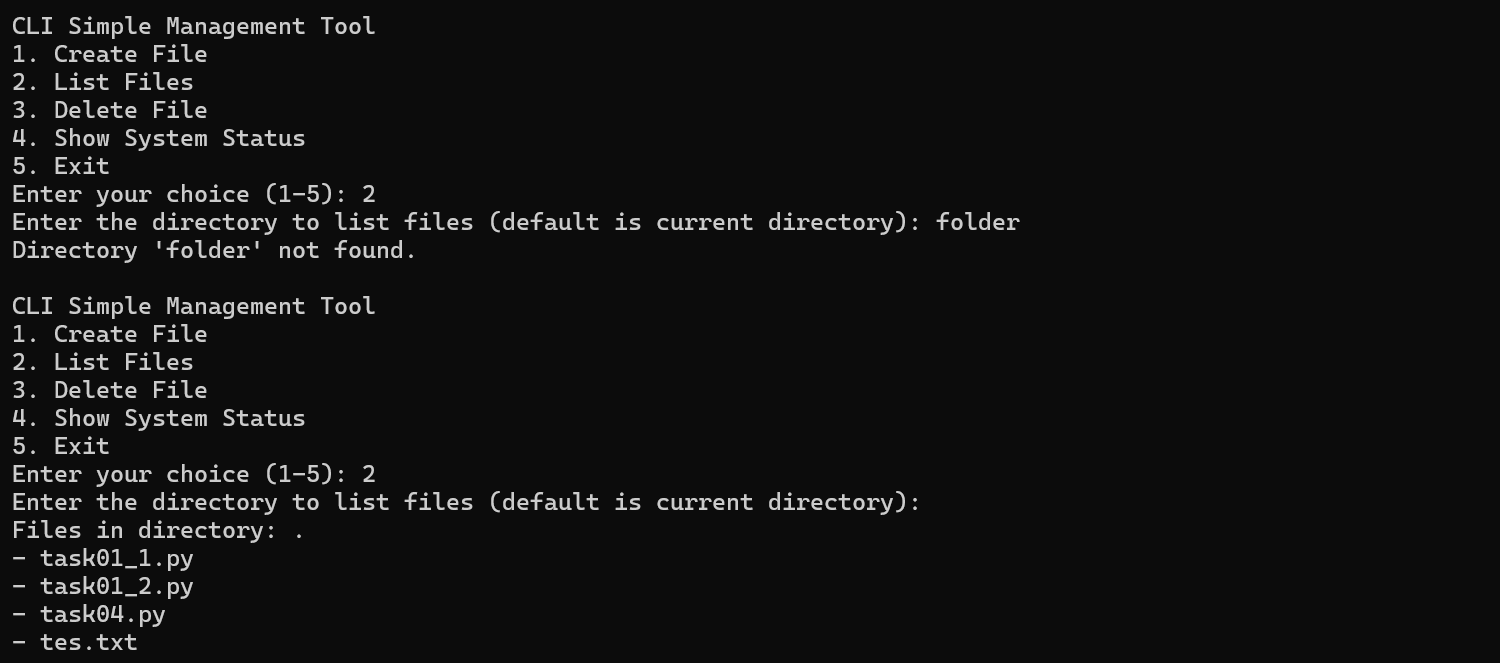
\includegraphics[width=0.9\textwidth]{asset/a4-output-2.png}
            \caption{Gambar 4: Menampilkan daftar \textit{file} dalam direktori}
            \label{fig:a4-output-2}
        \end{figure}
        \begin{figure}[htbp]
            \centering
            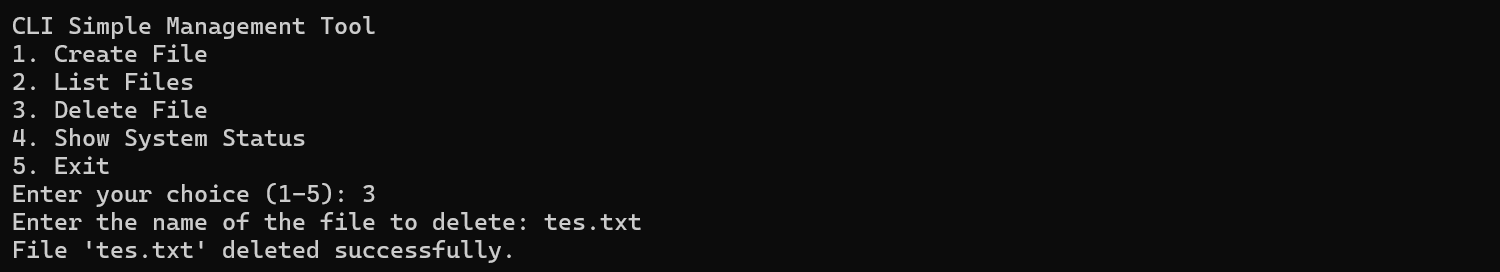
\includegraphics[width=0.9\textwidth]{asset/a4-output-3.png}
            \caption{Gambar 5: Menghapus \textit{file} bernama 'tes.txt'}
            \label{fig:a4-output-3}
        \end{figure}
        \begin{figure}[htbp]
            \centering
            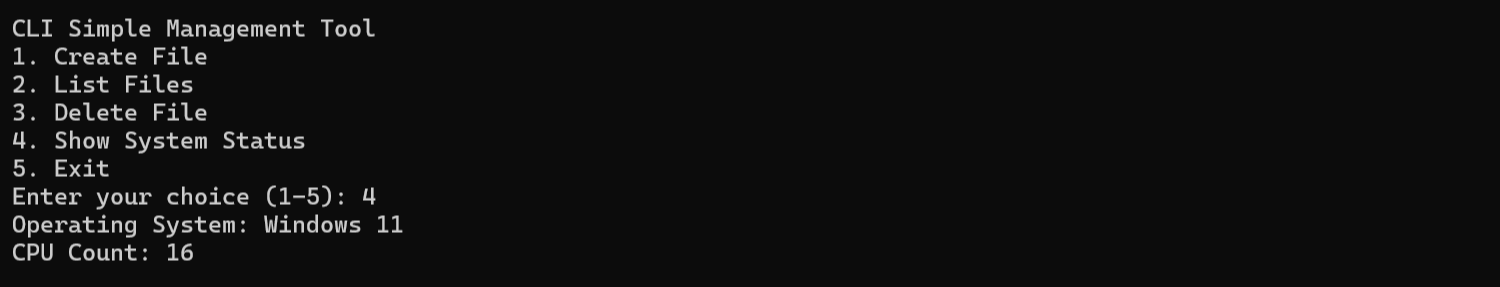
\includegraphics[width=0.9\textwidth]{asset/a4-output-4.png}
            \caption{Gambar 6: Menampilkan status sistem sederhana}
            \label{fig:a4-output-4}
        \end{figure}
        \begin{figure}[htbp]
            \centering
            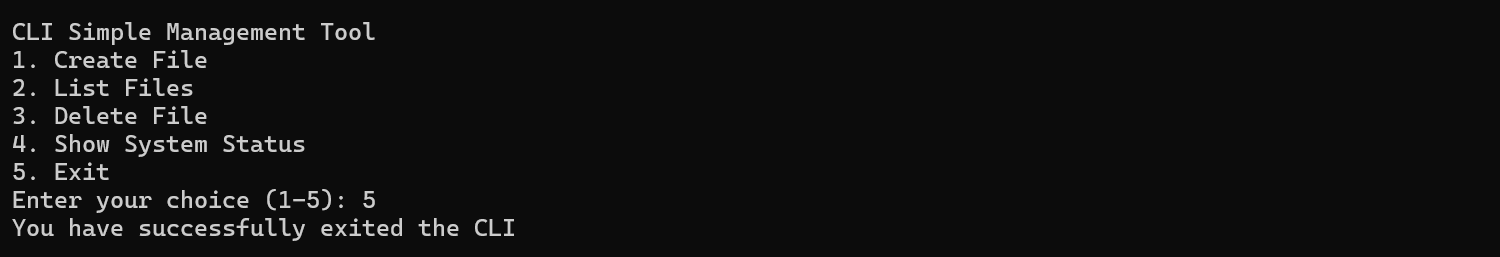
\includegraphics[width=0.9\textwidth]{asset/a4-output-5.png}
            \caption{Gambar 7: Keluar dari program}
            \label{fig:a4-output-5}
        \end{figure}

\subsection{Assignment 5: File System Access}
In this assignment, students implemented file system access routines, including:
\begin{itemize}
    \item File creation and deletion
    \item Reading from and writing to files
    \item Navigating directories and managing file permissions
\end{itemize}

\section{Conclusion}
The first half of the course introduced core operating system concepts, including process management, scheduling, multithreading, and file system access. These topics provided a foundation for more advanced topics to be covered in the second half of the course.

\end{document}